\documentclass[a4paper,10pt]{article}

\usepackage{url}

\usepackage[T1]{fontenc}
\usepackage[utf8]{inputenc}
\usepackage[spanish, es-tabla]{babel}

\clubpenalty=10000
\widowpenalty=10000

\usepackage[gen]{eurosym}

\usepackage{xcolor}
\usepackage{setspace}
\usepackage{float}
\usepackage{biblatex}
\addbibresource{fuentes.bib}
\setlength{\parindent}{0cm}
\usepackage{amsmath, amssymb}

% Listados de código
\usepackage{minted}
\usepackage{caption}
\newenvironment{code}{\captionsetup{type=listing}}{}
% \SetupFloatingEnvironment{listing}{name=Source Code}
\renewcommand{\listingscaption}{Código}
\BeforeBeginEnvironment{minted}{\vspace{-.3cm}}
\AfterEndEnvironment{minted}{\vspace{-.3cm}}

\usepackage{csquotes}

\renewcommand{\it}[1]{\textit{#1}}
\renewcommand{\bf}[1]{\textbf{#1}}
\renewcommand{\tt}[1]{\texttt{#1}}


\usepackage{booktabs} % Allows the use of \toprule, \midrule and \bottomrule in tables for horizontal lines
\usepackage{graphicx}
\graphicspath{{imagenes/}{../imagenes/}} % Declara dos paths, uno con respecto a este documento y otro respecto a la carpeta secciones

\parskip=0.4cm % Distancia entre párrafos

\usepackage[margin=3cm, headheight=13.6pt]{geometry}
 \usepackage{fancyhdr}
\fancyhf{}
\lhead{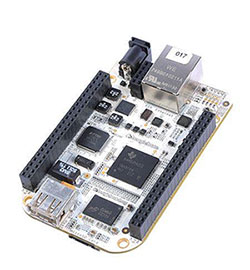
\includegraphics[width=0.5cm]{product_beaglebone.jpg}}
\fancyhead[C]{\emph{Sistemas Empotrados 2 -- 2020-21}}
\rhead{\emph{Práctica 4}}
\fancyfoot[C]{\thepage}

\usepackage{subfiles} % Permite incluir ficheros .tex en el texto

\usepackage{hyperref} % Hace que el índice sean hiperenlaces al documento

\begin{document}

\begin{titlepage}
    \centering
    
\includegraphics[width=1 cm]{logoUZ.jpg}
    
    \textsc{\large Universidad de Zaragoza}
    \rule{\textwidth}{1.6pt}\vspace*{-\baselineskip}\vspace*{2pt} % Thick horizontal rule
    \rule{\textwidth}{0.4pt} % Thin horizontal rule
    
    \vfill
    
    {\LARGE \scshape Sistemas Empotrados 2}
                
    \vspace{2cm}            

    {\bfseries \Huge Práctica 4}
    
    \vspace{.5cm} 
    
    {\bfseries \Large Medida de latencia de interrupción en Linux}
    
    \vspace{3cm}    
    
   

    {\scshape Autor:}


    \vspace{0.2cm}
    
    \large
    \begin{tabular}{c l l}
    \large             & Adrián Martín Marcos       & 756524 \\
     \end{tabular}

    \vfill
    
    \large{Zaragoza, España}
    
    {Curso 2020\,--\,2021}

    \vfill

    
\includegraphics[width=5.0cm]{EINA.png}
   
\end{titlepage}

\pagenumbering{Roman}


\vspace*{2cm}

\begin{spacing}{0.1}
\tableofcontents
\end{spacing}
%\listoffigures
%\listoftables

\pagebreak

\setcounter{page}{1}
\pagenumbering{arabic}

\pagestyle{fancy}

\subfile{secciones/1-configuracion-kernel}

\clearpage{}
\newpage

\subfile{secciones/2-primer-apartado}

\clearpage{}
\newpage

\subfile{secciones/3-segundo-apartado}

\clearpage{}
\newpage
\nocite{*}
\addcontentsline{toc}{section}{Referencias} % Añade en índice
\printbibliography

\end{document}


